\section{Geo-zones}
As the first example for GIS web view component possibilities Geo-zone visual representation can be used.
Geo-zones represent simple geographical polygons that can ``guard'' machine movements and help in storing
intersection events. They can be used to determine whether machine is in the right place in particular time
or whether the route is performing well.

After running the query for the first time by clicking on the Run button all existing Geo-zones are shown 
as small purple graphic primitives. They are also fitted to the bounds of visible map view. One can also 
do manual Fit To Bounds action by clicking appropriate button:
\begin{figure}[!htp]
\centering
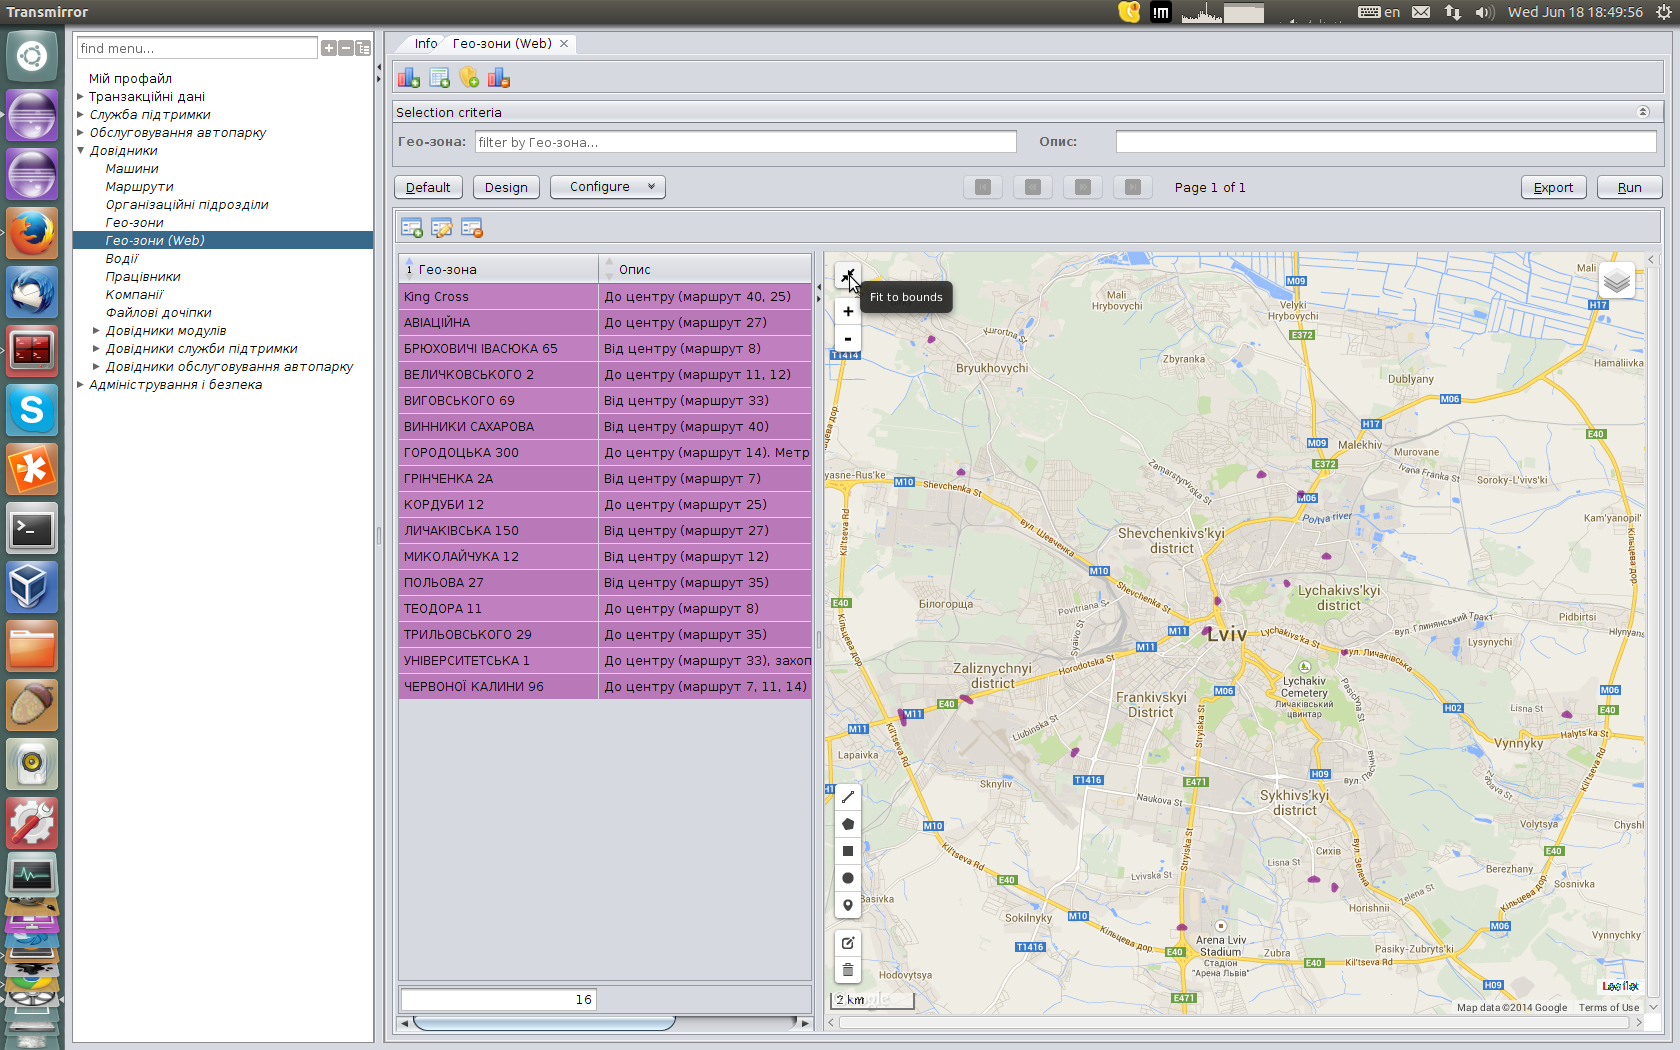
\includegraphics[width=16cm]{chapters/01-geozones/images/01-all-geo-zones-using-fit-to-bounds-button.png}
\caption{all-geo-zones-using-fit-to-bounds-button}\label{fig:01}
\end{figure}
Zooming can be done traditionally with mouse wheel button but also shift+selection works as a convenient 
zooming method:
\begin{figure}[!htp]
\centering
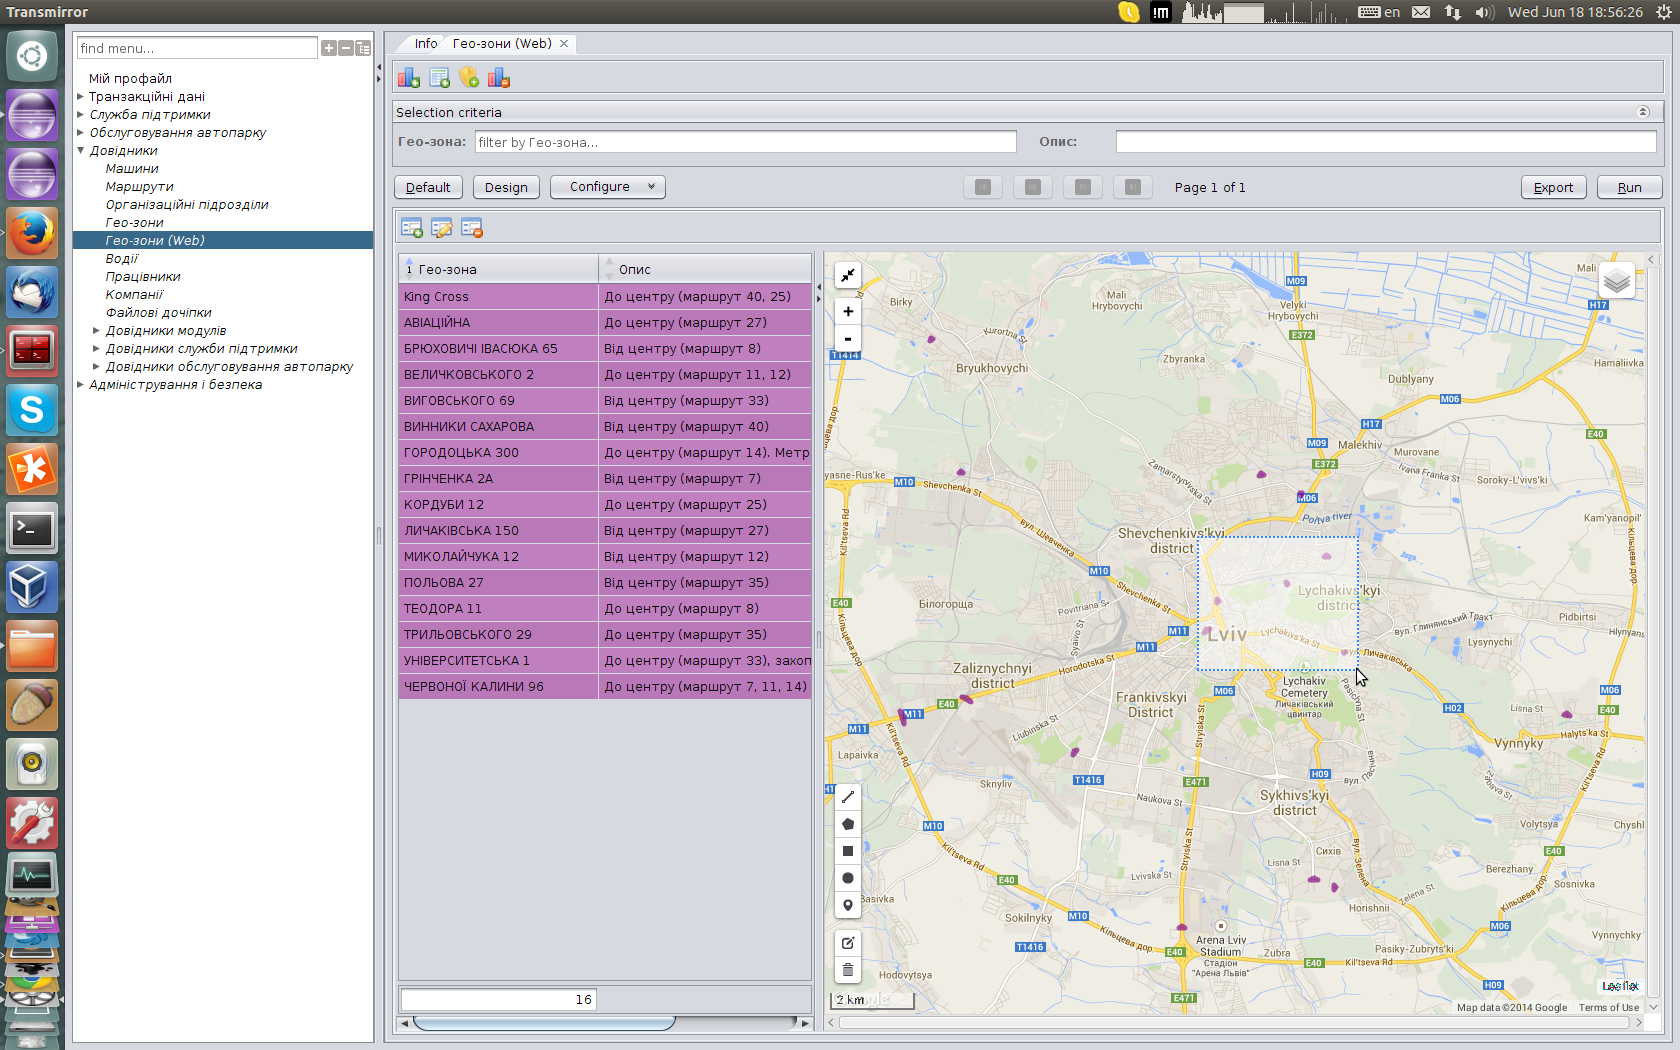
\includegraphics[width=16cm]{chapters/01-geozones/images/02-part-of-geo-zones-using-shift+selection-zoom.png}
\caption{part-of-geo-zones-using-shift+selection-zoom}\label{fig:02}
\end{figure}
The result of zooming shows that example Geo-zones has been represented as triangles. But the shapes are not 
limited only by triangles -- complex polygons or circles can be used as well.
\begin{figure}[!htp]
\centering
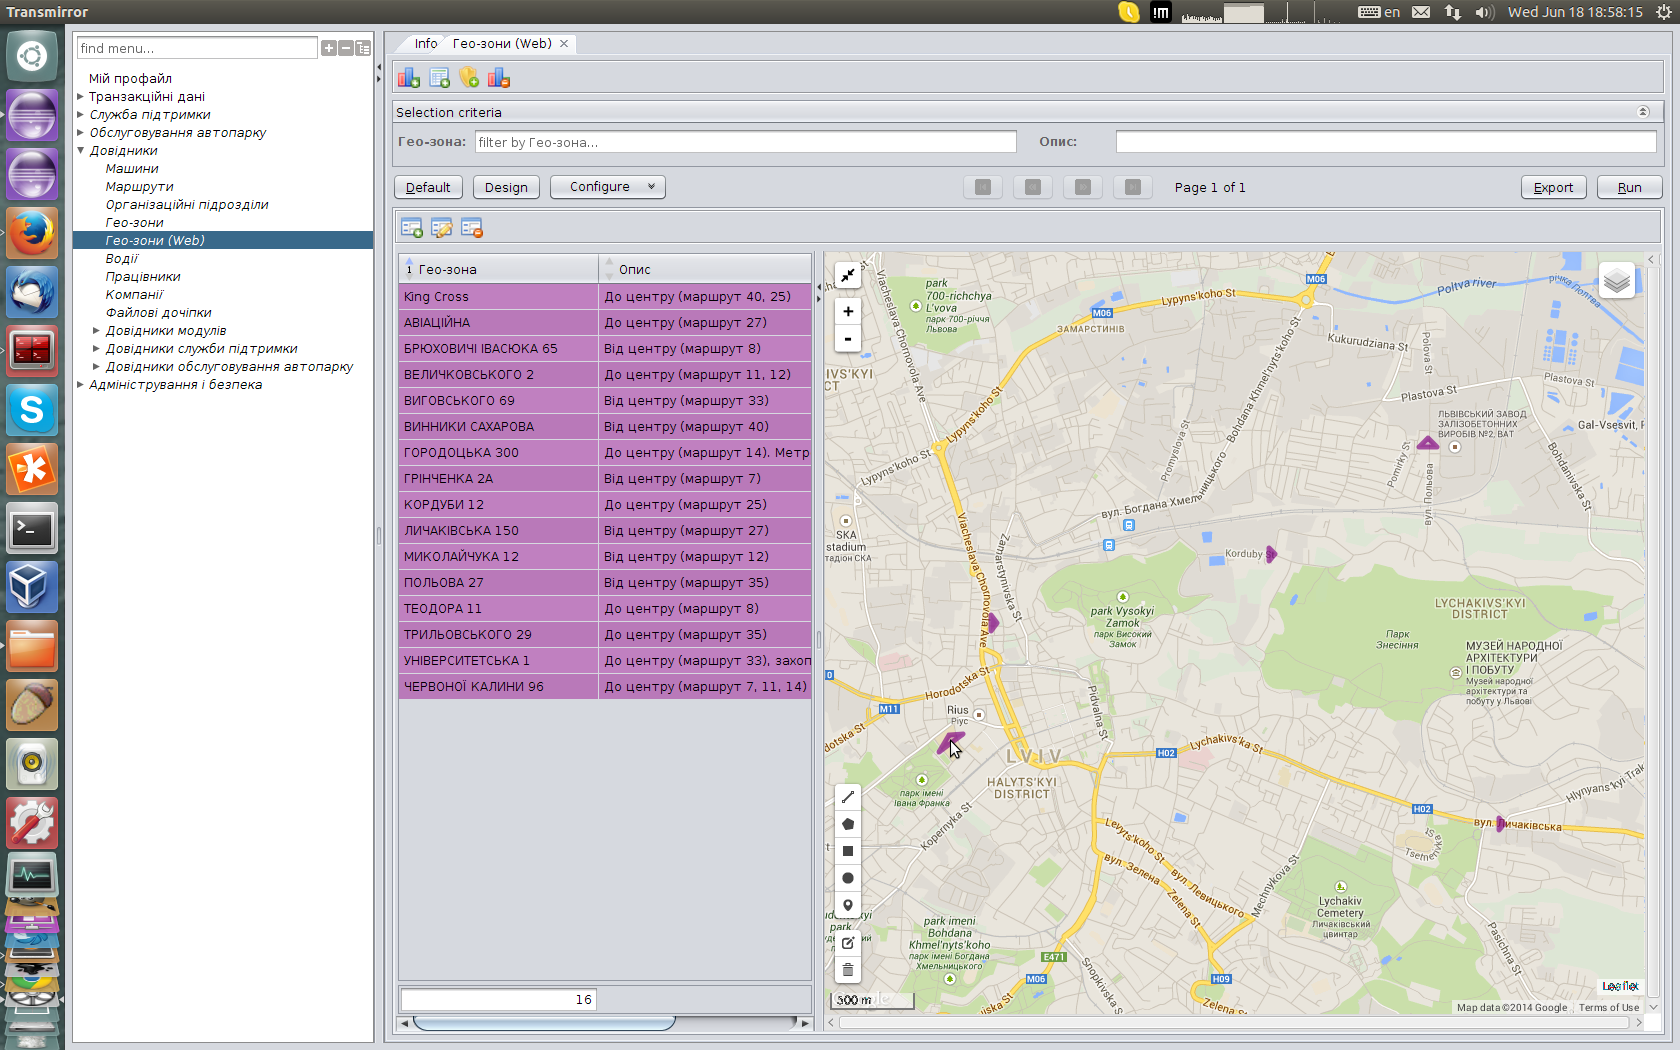
\includegraphics[width=16cm]{chapters/01-geozones/images/03-part-of-geo-zones-with-particular-item-selection-by-clicking.png}
\caption{part-of-geo-zones-with-particular-item-selection-by-clicking}\label{fig:03}
\end{figure}
Clicking on triangle will fit it to the bounds of the map and will show the detailed popup information. The table 
also will synchronise with the selected item (appropriate table row will also be selected):
\begin{figure}[!htp]
\centering
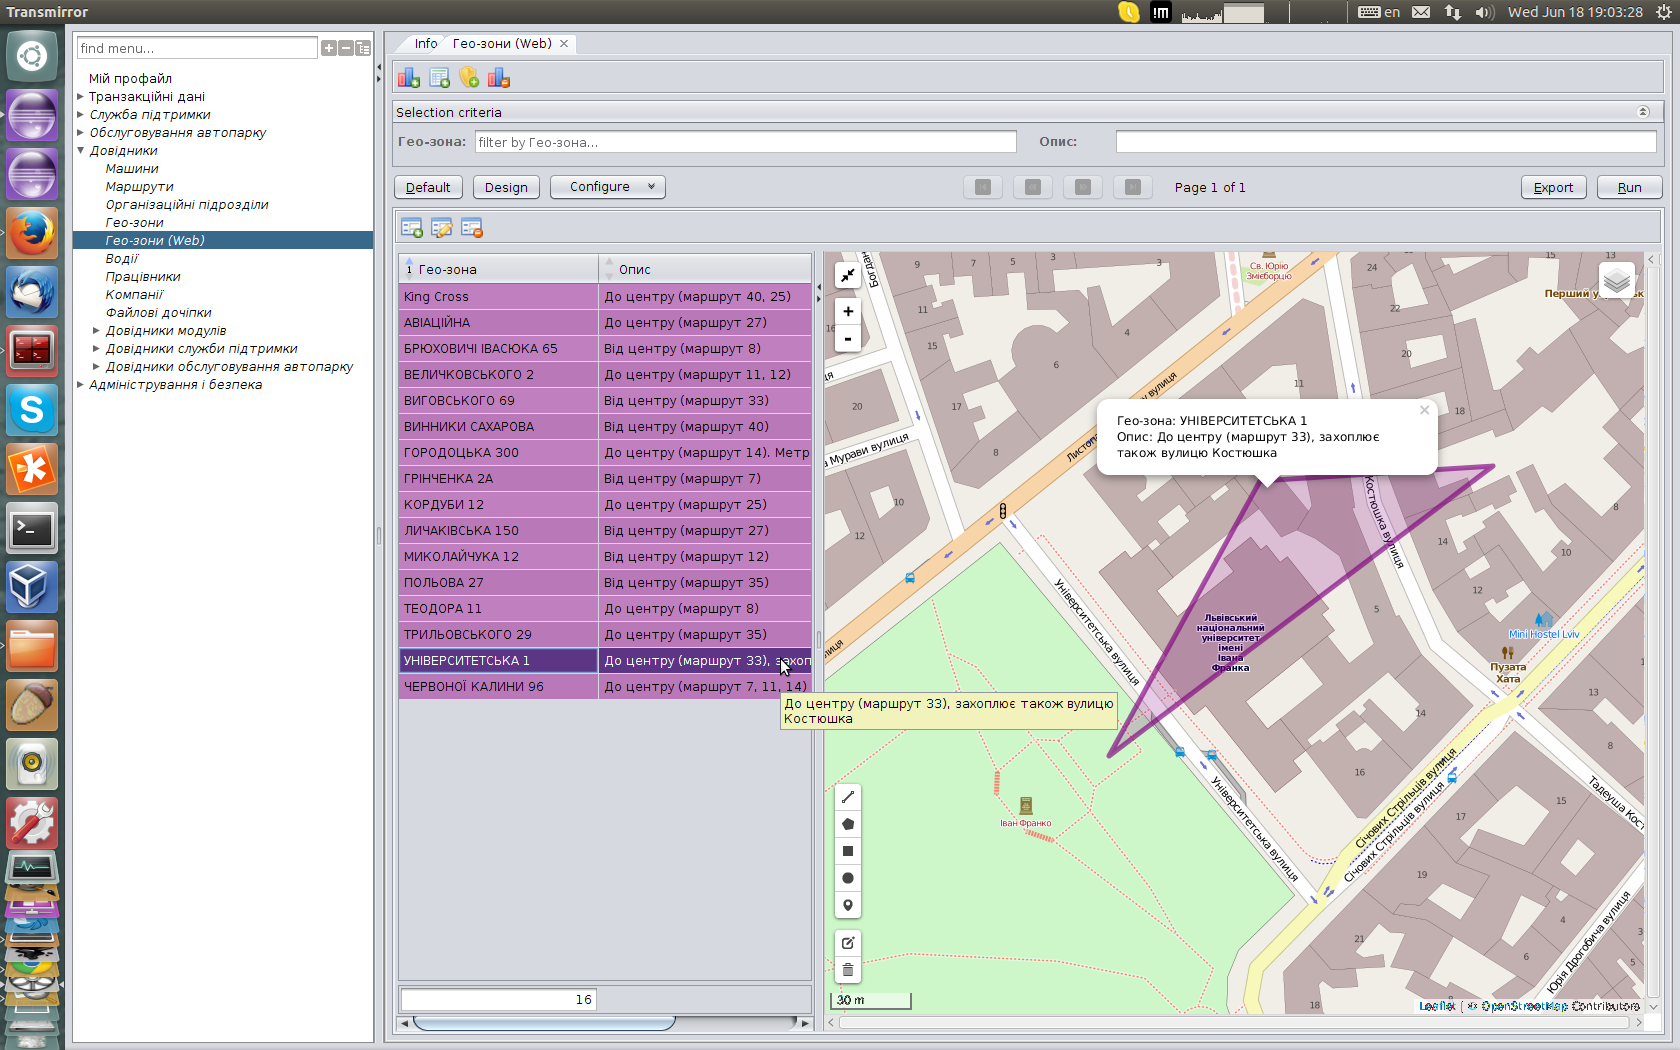
\includegraphics[width=16cm]{chapters/01-geozones/images/04-selected-geo-zone-and-synchronised-with-grid.png}
\caption{selected-geo-zone-and-synchronised-with-grid}\label{fig:04}
\end{figure}
Editing of Geo-zones is also supported by dragging polygon corners. Appropriate shape can be formed with 
arbitrary number of corners. The changes can be simply discarded if needed using ``Cancel" button or saved 
with ''Save" button:
\begin{figure}[!htp]
\centering
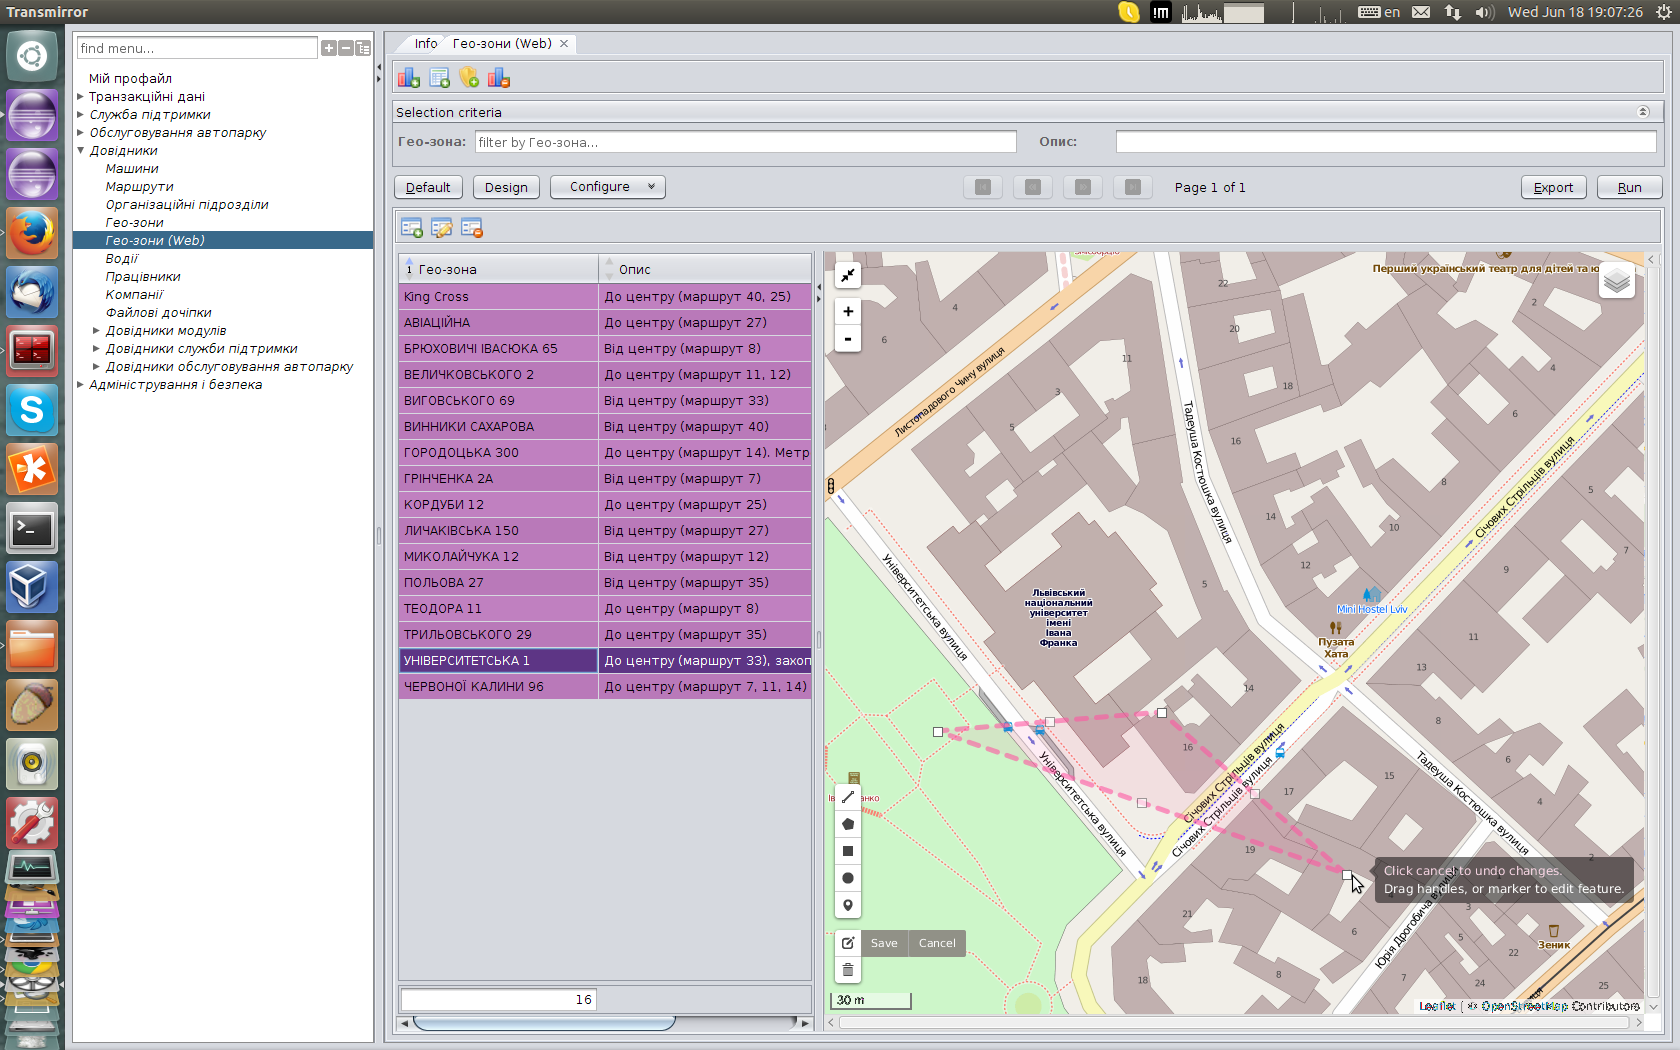
\includegraphics[width=16cm]{chapters/01-geozones/images/05-editing-geo-zone-using-graphical-interface.png}
\caption{editing-geo-zone-using-graphical-interface}\label{fig:05}
\end{figure}
The result of editing is a regular shape:
\begin{figure}[!htp]
\centering
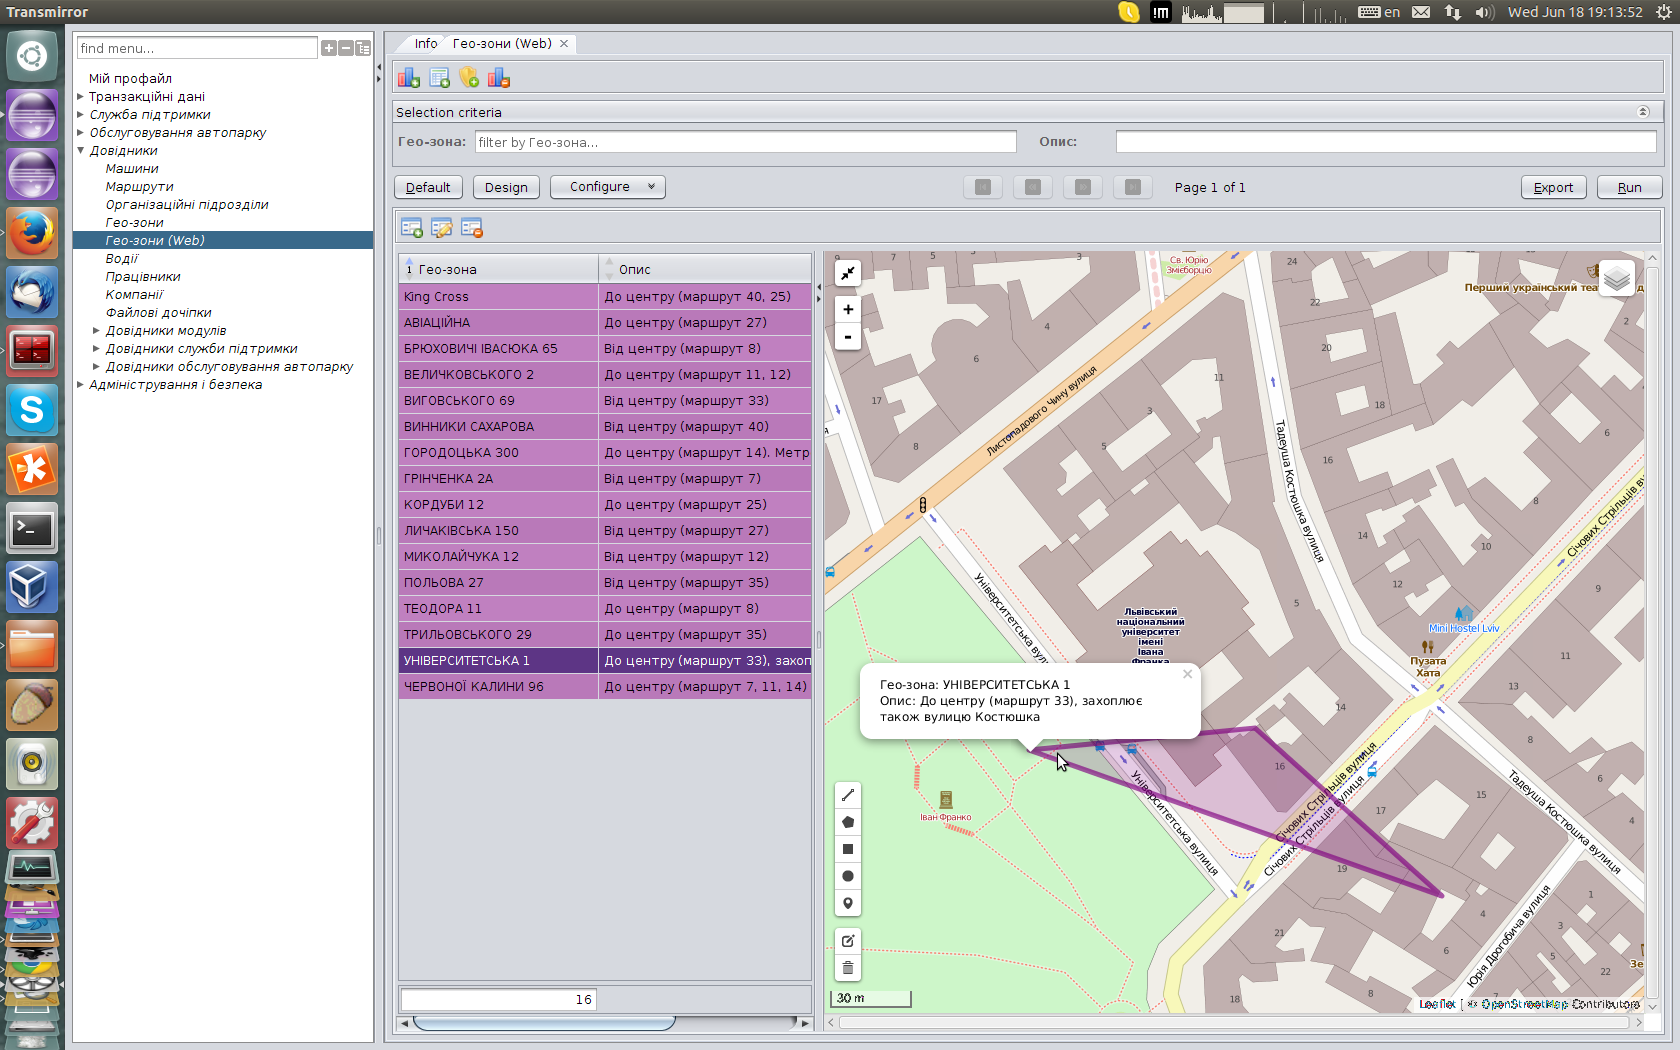
\includegraphics[width=16cm]{chapters/01-geozones/images/06-edited-geo-zone.png}
\caption{edited-geo-zone}\label{fig:06}
\end{figure}
Complex Geo-zones can be used including circles, rectangles or polygons:
\begin{figure}[!htp]
\centering
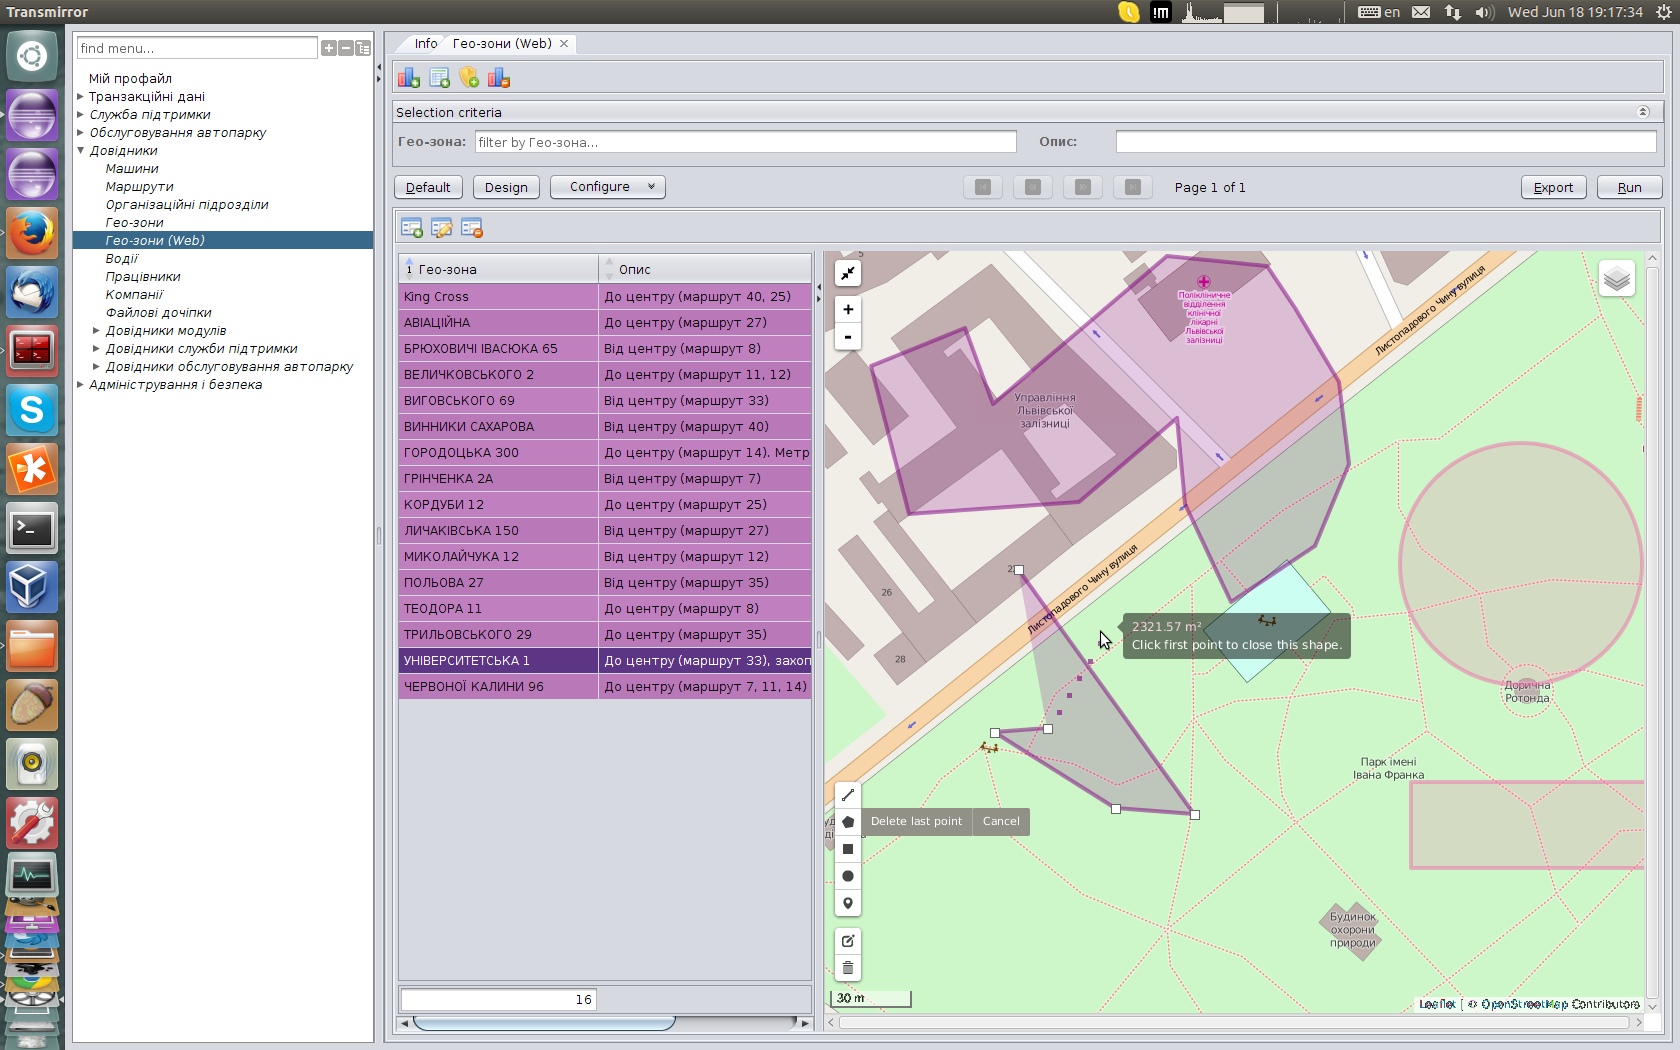
\includegraphics[width=16cm]{chapters/01-geozones/images/07-creating-new-complex-geo-zones.png}
\caption{creating-new-complex-geo-zones}\label{fig:07}
\end{figure}
Validation for the shape is necessary to make possible only meaninful Geo-zones (the edges should not cross):
\begin{figure}[!htp]
\centering
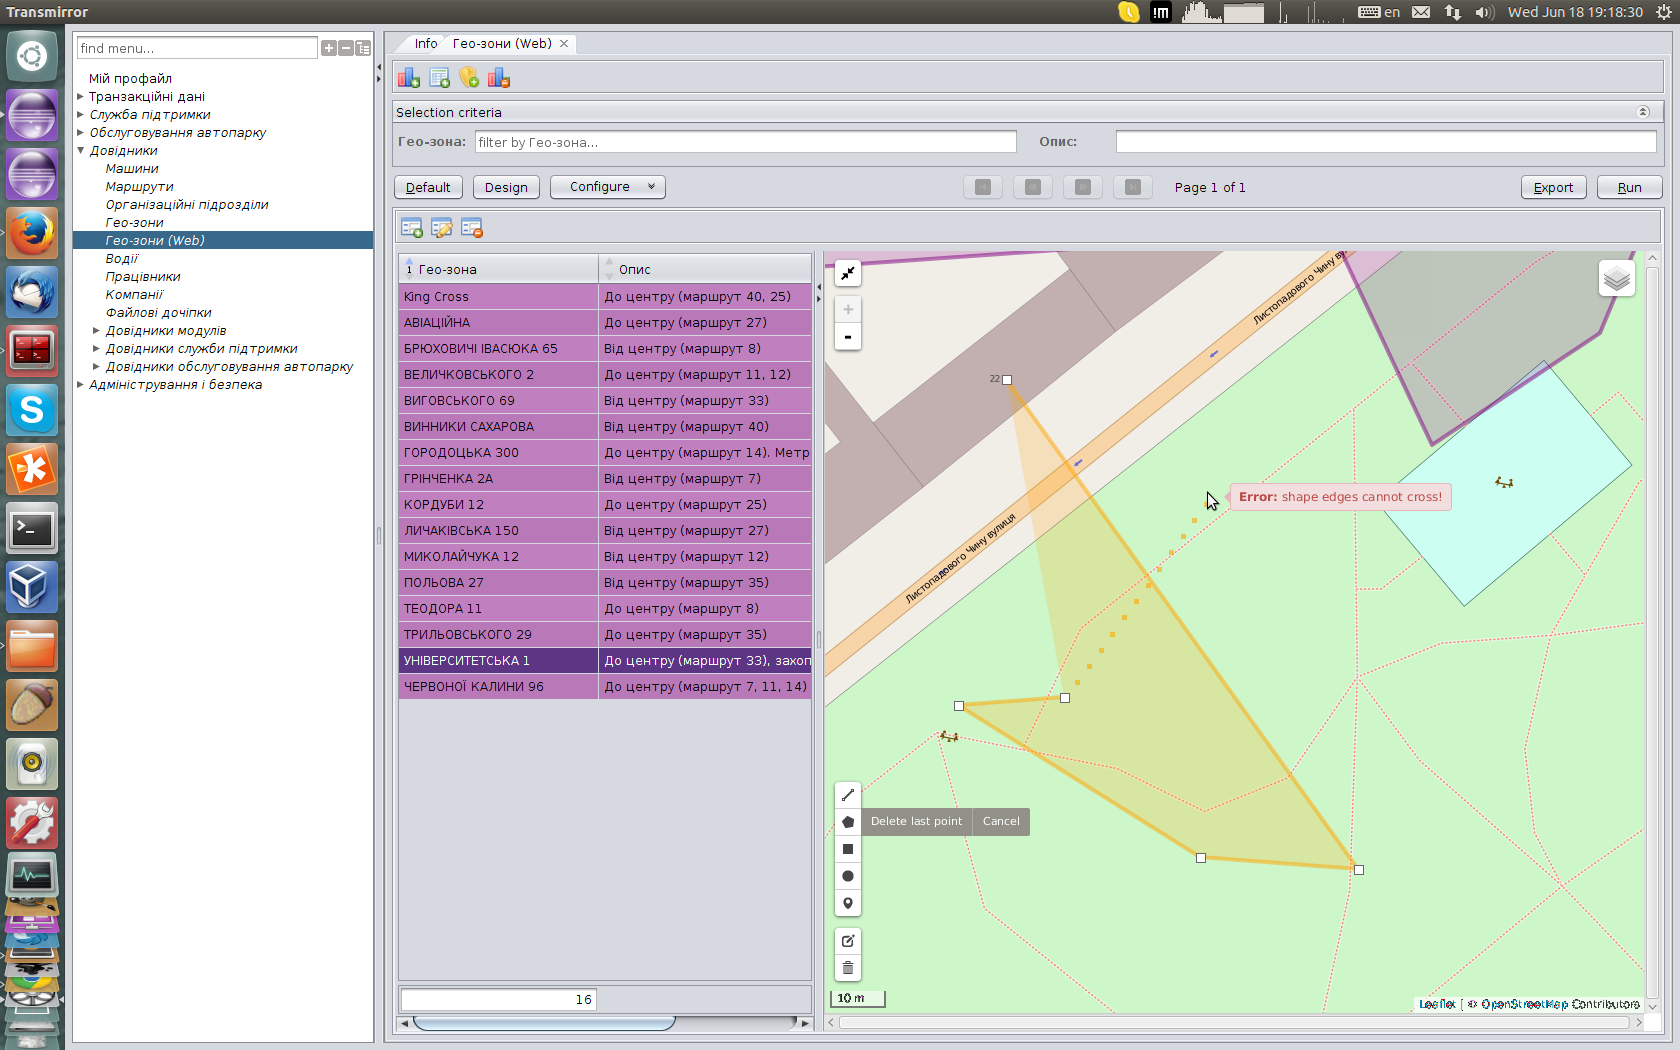
\includegraphics[width=16cm]{chapters/01-geozones/images/08-validation-for-complex-polygonial-geozone.png}
\caption{validation-for-complex-polygonial-geozone}\label{fig:08}
\end{figure}
Map service changing is easily done by clicking on right top button. Basically tile services are not
limited only by OpenStreetMap, Google, Yandex and Landscape (but at this stage only those are supported): 
\begin{figure}[!htp]
\centering
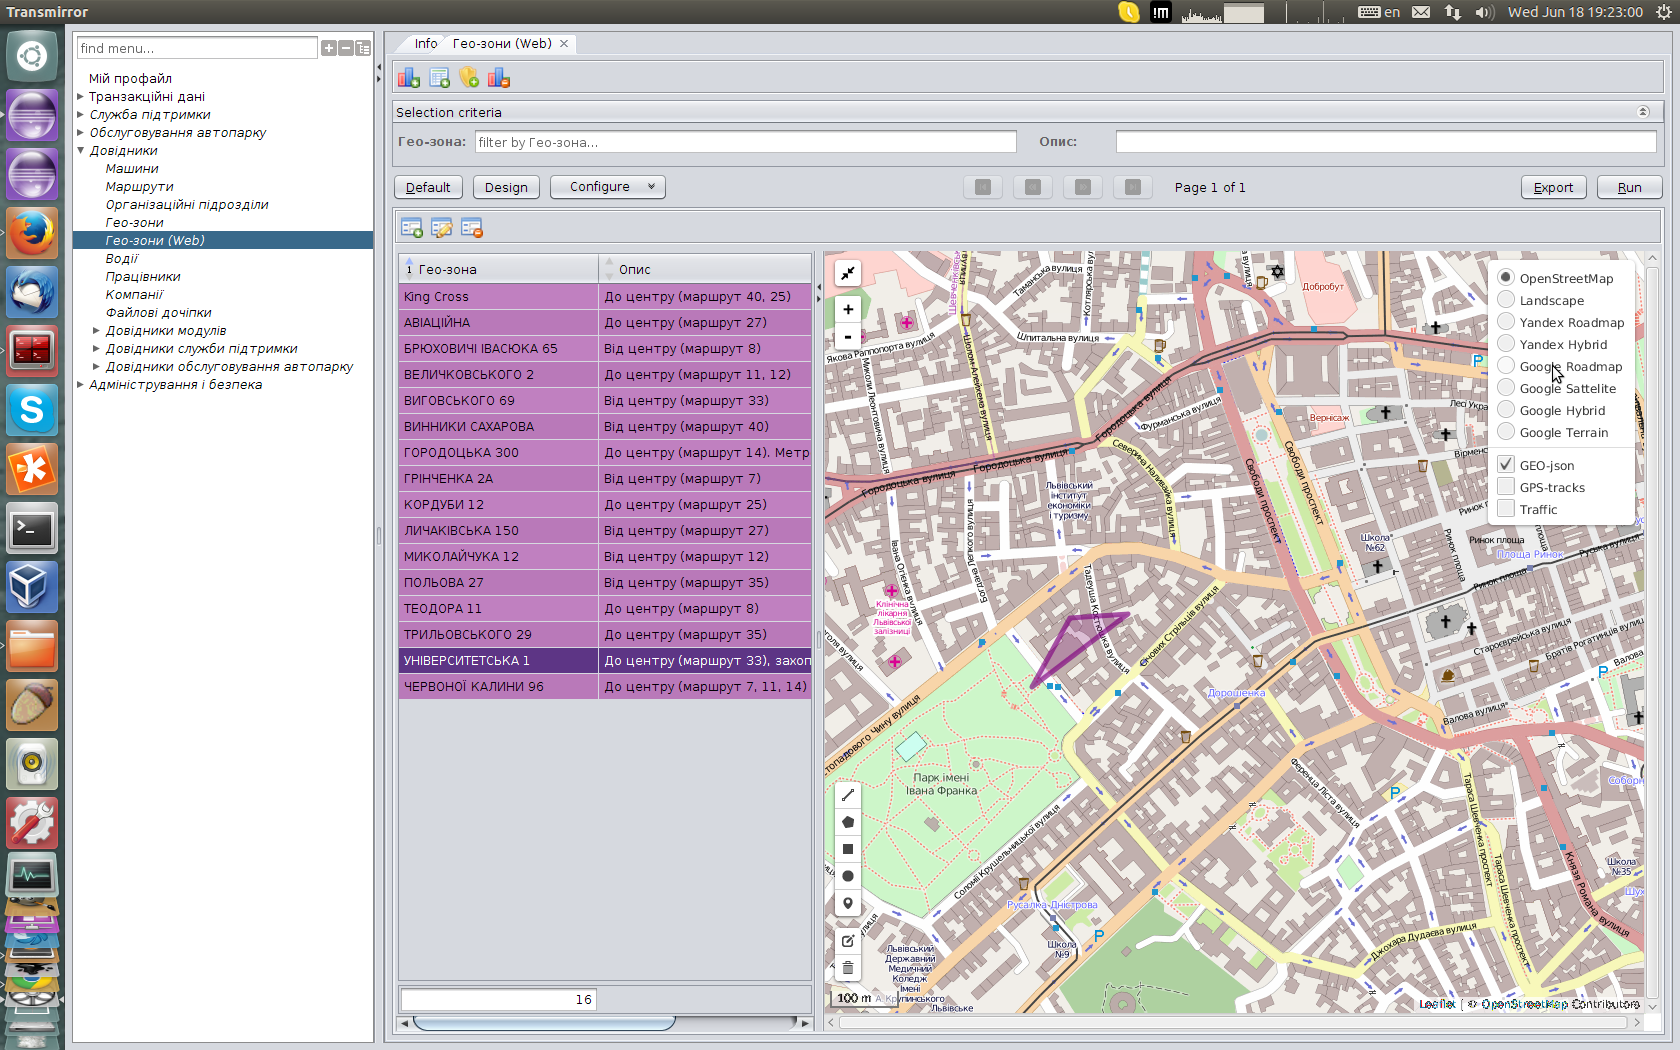
\includegraphics[width=16cm]{chapters/01-geozones/images/09-changing-map-tiling-service.png}
\caption{09-changing-map-tiling-service}\label{fig:09}
\end{figure}

\begin{figure}[!htp]
\centering
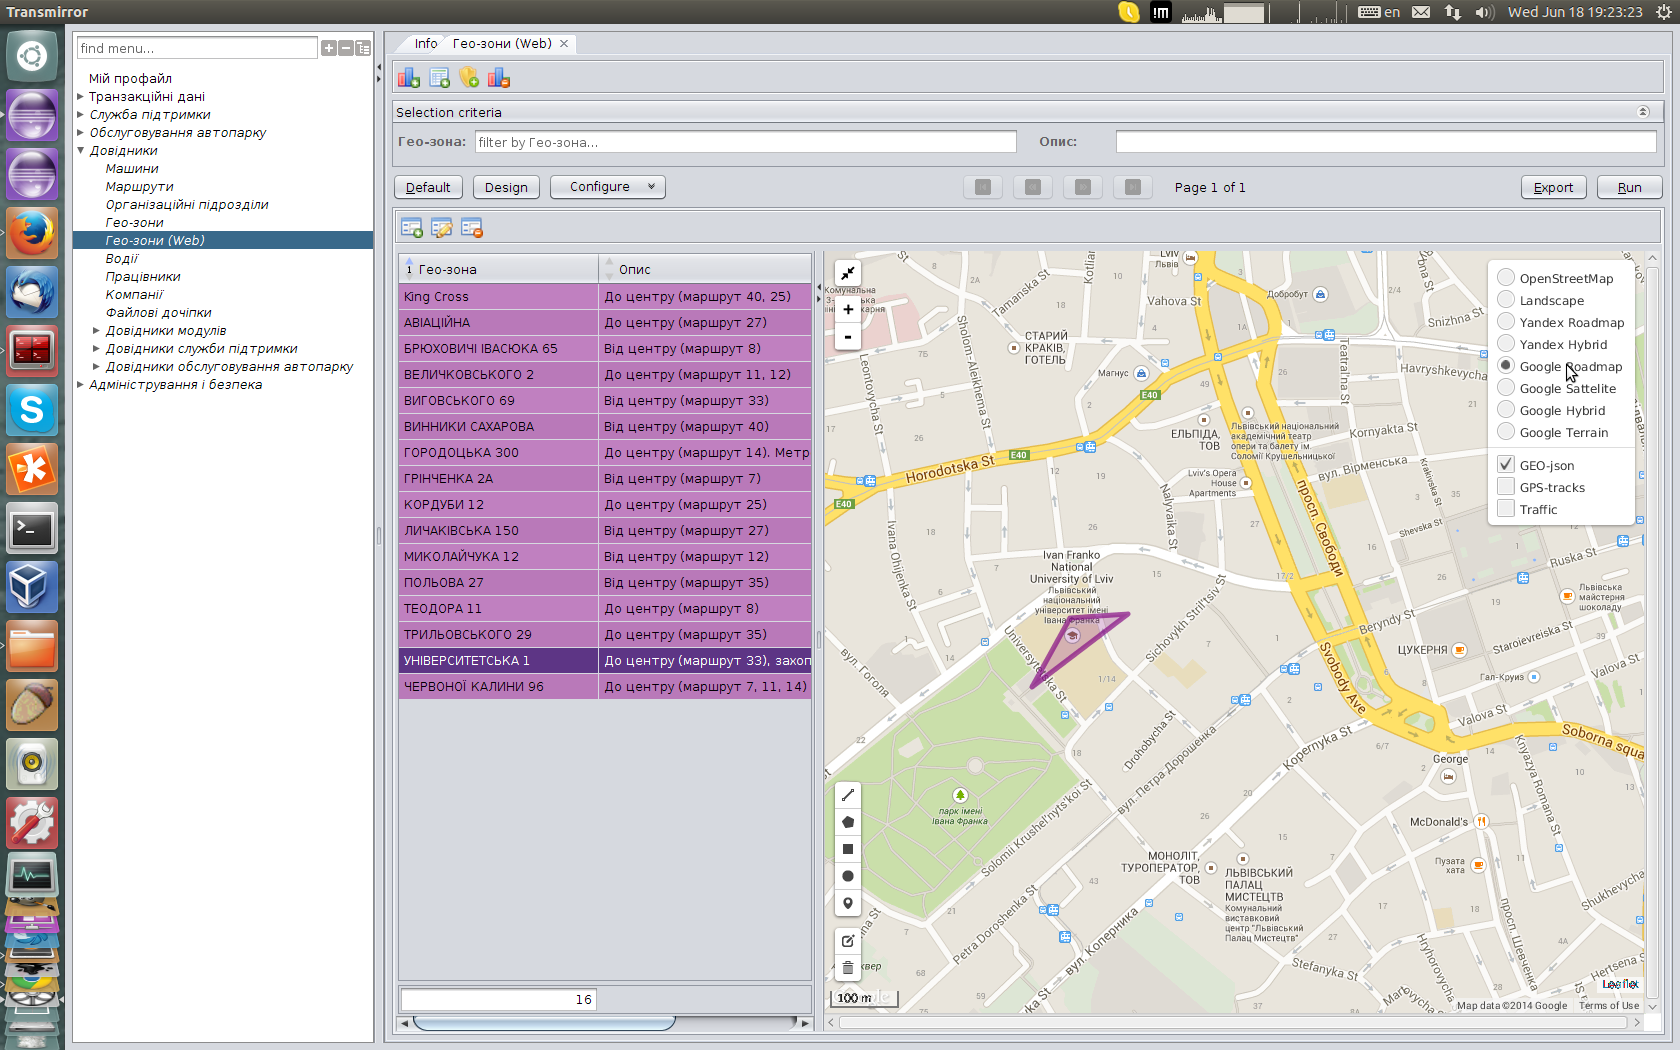
\includegraphics[width=16cm]{chapters/01-geozones/images/10-changed-map-tiling-service.png}
\caption{changed-map-tiling-service}\label{fig:10}
\end{figure}